\documentclass[../DoAn.tex]{subfiles}
\begin{document}
Chương này có độ dài từ 9 đến 11 trang.

Với phương pháp phân tích thiết kế hướng đối tượng, sinh viên sử dụng biểu đồ use case theo hướng dẫn của template này. Với các phương pháp khác, sinh viên trao đổi với giáo viên hướng dẫn để đổi tên và sắp xếp lại đề mục cho phù hợp. Ví dụ, thay vì sử dụng biểu đồ use case, sinh viên đi theo hướng tiếp cận Agile có thể dùng User Story.


\textbf{Lưu ý}: Mỗi chương nên có thêm 1 đoạn mở đầu chương và kết thúc chương, mở đầu giới thiệu những nội dung sẽ trình bày trong chương, kết thúc tổng kết lại các nội dung đã trình bày

\section{Khảo sát hiện trạng}
\label{section:2.1}

Hiện nay trên thị trường đã có một số ứng dụng hỗ trợ việc tìm và đặt người lái hộ như: FastGo, ViSafe, GOCheap,...
Dưới đây là đánh giá về các ứng dụng này để tìm hiểu về các tính năng cũng như hạn chế của chúng:

\textbf{FastGo}: FastGo là một trong những ứng dụng thuê lái xe hộ khi say được yêu thích hiện nay. 
Được phát triển bởi công ty cổ phần FastGo Việt Nam, app này cung cấp dịch vụ lái xe chuyên nghiệp và an toàn cho người sử dụng.
\begin{itemize}
    \item Ưu điểm:
      \begin{itemize}
        \item Giao diện đơn giản, dễ sử dụng
        \item Bảo mật thông tin cá nhân
        \item Tính năng đặt xe và theo dõi hành trình dễ dàng
        \item Hỗ trợ khách hàng 24/7
      \end{itemize}
    \item Hạn chế:
      \begin{itemize}
        \item Cần phải kết nối mạng ổn định
        \item Không có tính năng đón khách
      \end{itemize}
\end{itemize}

\textbf{ViSafe}: ViSafe là một ứng dụng thuê lái xe hộ khi say được phát triển bởi Công ty Cổ Phần An Toàn Giao Thông Việt Nam. App này nhắm đến việc cung cấp dịch vụ an toàn và chất lượng cho người sử dụng.
\begin{itemize}
    \item Ưu điểm:
      \begin{itemize}
        \item Giao diện đơn giản, dễ sử dụng
        \item Bảo mật thông tin cá nhân
        \item Hỗ trợ khách hàng 24/7
        \item Đa dạng tính năng
      \end{itemize}
    \item Hạn chế:
      \begin{itemize}
        \item Không có tính năng theo dõi hành trình
      \end{itemize}
\end{itemize}

\textbf{GOCheap}: GOCheap là một trong những app đặt lái xe hộ khi say tuyệt vời nhất ở thời điểm hiện tại. Ứng dụng này được phát triển và quản lý bởi Công ty TNHH GOCheap. Ứng dụng này nhắm đến mục tiêu cung cấp dịch vụ thuê lái xe hộ chất lượng và uy tín nhất cho người dùng.
\begin{itemize}
    \item Ưu điểm:
      \begin{itemize}
        \item Tiện lợi, nhanh chóng
        \item Dịch vụ chất lượng
        \item Bảo mật tốt
        \item Hỗ trợ 24/7
      \end{itemize}
    \item Hạn chế:
      \begin{itemize}
        \item Giao diện chưa không thân thiện
      \end{itemize}
\end{itemize}


\section{Tổng quan chức năng}
\label{section:2.2}

\subsection{Biểu đồ use case tổng quát}
\label{subsection:2.2.1}
\begin{figure}[H]
    \centering
    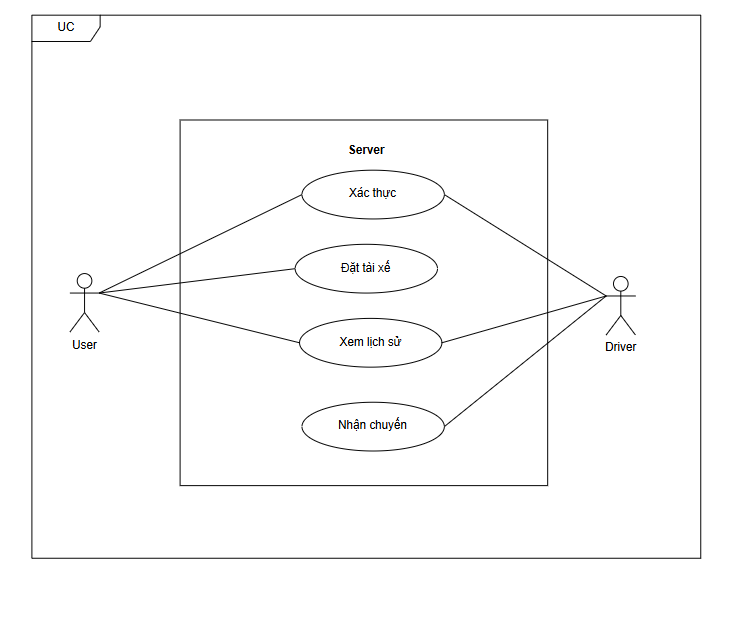
\includegraphics[width=0.8\textwidth]{Hinhve/Usecase_tong_quan.png}
    \caption{Biểu đồ use case tổng quát}
    \label{fig:use_case_total}
\end{figure}
Hệ thống gồm 2 tác nhân là User và Driver.
Để sử dụng các chức năng trong ứng dụng thì cả user và driver đều cần đăng nhập bằng số điện thoại và mật khẩu.
Hệ thống bao gồm các usecase chính sau (i) usecase xác thực: xử lý việc đăng nhập, đăng ký của người dùng; 
(ii) usecase đặt tài xế: tìm kiếm địa điểm, xem giá cước, chọn phương tiện, đặt tài xế;
(iii) usecase xem lịch sử: người dùng xem lại lịch sử các chuyến đi của mình;
(iv) usecase nhận chuyến: tài xế nhận được thông tin về chuyến đi, nhận hoặc hủy chuyến


\subsection{Biểu đồ use case phân rã Xác thực}
\label{subsection:2.2.2}
\begin{figure}[H]
  \centering
  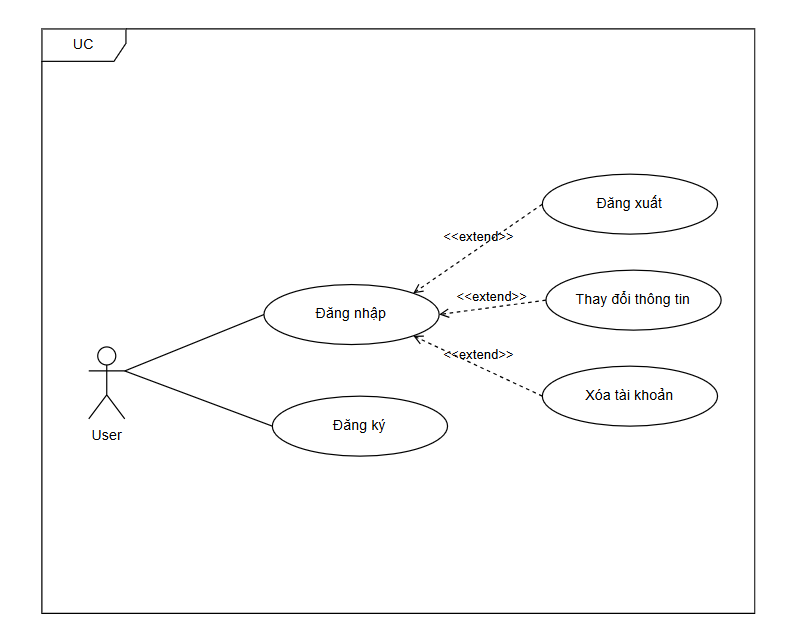
\includegraphics[width=0.8\textwidth]{Hinhve/Usecase_xac_thuc.png}
  \caption{Biểu đồ usecase Xác thực}
  \label{fig:use_case_xac_thuc}
\end{figure}
Usecase Xác thực bao gồm những chức năng chính sau (i) đăng nhập: người dùng nhập số điện thoại và mật khẩu để đăng nhập vào hệ thống, (ii) đăng ký: người dùng nhập các thông tin bắt buộc để đăng ký, (iii) đăng xuất: Đăng xuất khỏi tài khoản đang được đăng nhập, (iv) xóa tài khoản: người dùng xóa tài khoản của mình và phải đăng ký hoặc đăng nhập tài khoản khác để sử dụng hệ thống, (v) thay đổi thông tin cá nhân: thay đổi các thông tin như họ tên, email, mật khẩu.

\subsection{Biểu đồ use case phân rã Đặt tài xế}
\label{subsection:2.2.3}
\begin{figure}[H]
  \centering
  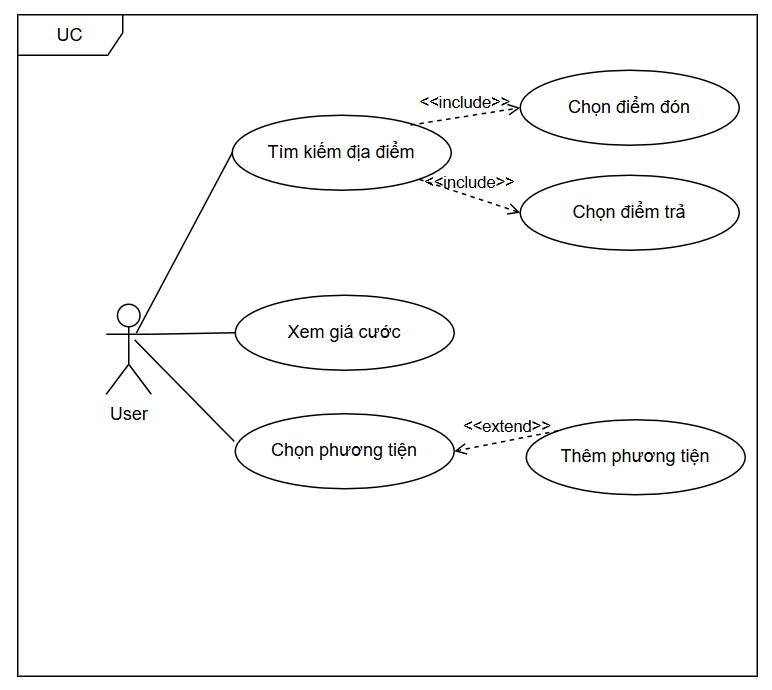
\includegraphics[width=0.8\textwidth]{Hinhve/Usecase_dat_tai_xe.png}
  \caption{Biểu đồ usecase Đặt tài xế}
  \label{fig:use_case_dat_tai_xe}
\end{figure}
Usecase Đặt tài xế bao gồm những chức năng chính sau (i) tìm kiếm địa điểm: người dùng nhập địa điểm để tìm kiếm, (ii) xem giá cước: người dùng xem giá cước của các chuyến đi, (iii) chọn phương tiện: người dùng chọn phương tiện để đặt chuyến, (iv) tìm tài xế: người dùng tìm kiếm tài xế cho chuyến đi, (v) thêm phương tiện: người dùng thêm phương tiện họ cần lái hộ, (vi) chọn phương tiện: người dùng chọn phương tiện cần lái hộ

\subsection{Quy trình nghiệp vụ}
\label{subsection:2.2.3}
Nếu sản phẩm/hệ thống cần xây dựng có quy trình nghiệp vụ quan trọng/đáng chú ý, sinh viên cần mô tả và vẽ biểu đồ hoạt động minh họa quy trình nghiệp vụ đó. Sinh viên lưu ý đây không phải là luồng sự kiện của từng use case, mà là luồng hoạt động kết hợp nhiều use case để thực hiện một nghiệp vụ nào đó.

Ví dụ, một hệ thống quản lý thư viện có quy trình nghiệp vụ mượn trả với mô tả sơ bộ như sau: Sinh viên làm thẻ mượn, sau đó sinh viên đăng ký mượn sách, thủ thư cho mượn, và cuối cùng sinh viên trả lại sách cho thư viện. Một hệ thống có thể có một vài quy trình nghiệp vụ quan trọng như vậy.
\section{Đặc tả chức năng}
\label{section:2.3}
Sinh viên lựa chọn từ 4 đến 7 use case quan trọng nhất của đồ án để đặc tả chi tiết. Mỗi đặc tả bao gồm ít nhất các thông tin sau: (i) Tên use case, (ii) Luồng sự kiện (chính và phát sinh), (iii) Tiền điều kiện, và (iv) Hậu điều kiện. Sinh viên chỉ vẽ bổ sung biểu đồ hoạt động khi đặc tả use case phức tạp.
\subsection{Đặc tả use case A}
\hfill
\subsection{Đặc tả use case B}
\hfill

\section{Yêu cầu phi chức năng}
\label{section:2.4}
Trong phần này, sinh viên đưa ra các yêu cầu khác nếu có, bao gồm các yêu cầu phi chức năng như hiệu năng, độ tin cậy, tính dễ dùng, tính dễ bảo trì, hoặc các yêu cầu về mặt kỹ thuật như về CSDL, công nghệ sử dụng, v.v.


%%%%%%%%%%%%%%%%%%%%%%%%%%%%%%%%%%%

\end{document}